\chapter{System Overview}
This report describes the working version of SWIM2 and its component modules, including data and calibration. This introduction describes the overall simulation system. It defines terms used often in the report, as well as the general calibration approach used in model development. The following chapters describe the individual model components. Within each discussion of them there are sections describing its design, to include equations and processes used. The estimation or synthesis of parameters and their values are described, as well as required model inputs. Sections describing the calibration process and outcomes are also included for each component.  

\section{Introduction}
The Oregon StateWide Integrated Model (SWIM2) is an integrated land use transport model covering the entire State of Oregon. It is a second generation model, drawing on previous work done on the first generation statewide model (SWIM1) and the Eugene-Springfield UrbanSim Model. The SWIM1 model \citep{parsons99} was a customized version of the TRANUS software\footnote{\url{http://www.tranus.com/tranus-english}}. SWIM2 is a more disaggregate and complex customized framework that combines a PECAS spatial allocation model with activity-based micro-simulation transport models. SWIM2 augments the SWIM1 Model in more complex applications of Oregon statewide policy and investment decisions. Future SWIM2 model upgrades will be driven by policy application needs.

The development of both the first and second generation models was commissioned by the Oregon Department of Transportation (ODOT) as part of its Transportation and Land Use Model Improvement Program (TLUMIP) within the larger Oregon Model Improvement Program (OMIP). The model development has been undertaken by a series of teams led by Parsons Brinckerhoff, with HBA Specto, EcoNorthwest and The University of Washington playing key roles as sub-contractors. The program has also been guided by an internationally prominent peer review panel.

The approach used in the development of SWIM2 has been to establish working versions and documentation of each of the modules shown in Figure \ref{fig:tlumip-schematic} (page \pageref{fig:tlumip-schematic}), before proceeding with full system integration. The preparation and testing of the software code, preparation of calibration and validation, establishing initial inputs and parameters and own-module calibration were completed first. Integration of the modules to run through time as a unit was completed next. Full model calibration of all modules in both a base year and trends overtime was completed and shared with the TLUMIP Peer Review Panel. Further calibration has and will continue to be performed as needed to match newer data and ensure the model is best equipped to address ODOT policy applications. 

The model is run in policy application mode for the period 2006-2030. The model steps through time in one-year intervals. The economic and spatial activities models --- the NED, SPG, ALD, and AA modules shown in Figure \ref{fig:tlumip-schematic} (page \pageref{fig:tlumip-schematic}) --- are run each year, while the transport models are only run every third year to reduce the time required to complete the entire simulation. The models were developed with an initial emphasis on reliability and ability to be easily understand and refactored. Subsequent versions of the models have been or will be tuned to achieved faster runtime performance.

% Removed Table 1, as it offered obsolete information at best

\section{Common modeling framework}
A great deal of data and information is shared by all components in the SWIM2 system. This includes model area category definitions, the Application Orchestrator (AO) module, and the overall calibration approach. Detailed descriptions of the user interface modules can be found in the SWIM2 User's Guide\footnote{https://github.io/tlumip/swim25/doc/userguide-v3.pdf}.

\subsection{Model area geography}\label{sec:model-area-geography}
The SWIM2 system operates at two geographic levels within the modeled area, show in Figure \ref{fig:swim2-model-area}. Both encompass 36 counties within Oregon and 39 counties in adjacent states. The latter is commonly referred to as to halo area of the model. The halo encompasses a roughly 50-mile buffer around Oregon. A system of 2,950 alpha zones (light and dark lines in Figure \ref{fig:swim2-model-area}) is the most disaggregate zone system. These include 12 external stations, show in Table \ref{tab:external-stations} and Figure \ref{fig:swim2-external-stations}. These external stations serve as gateways to the the six world markets used to represent the world beyond the halo.

\begin{figure}[!t]    % Figure 2.1 (although mis-captioned in original)
\centering
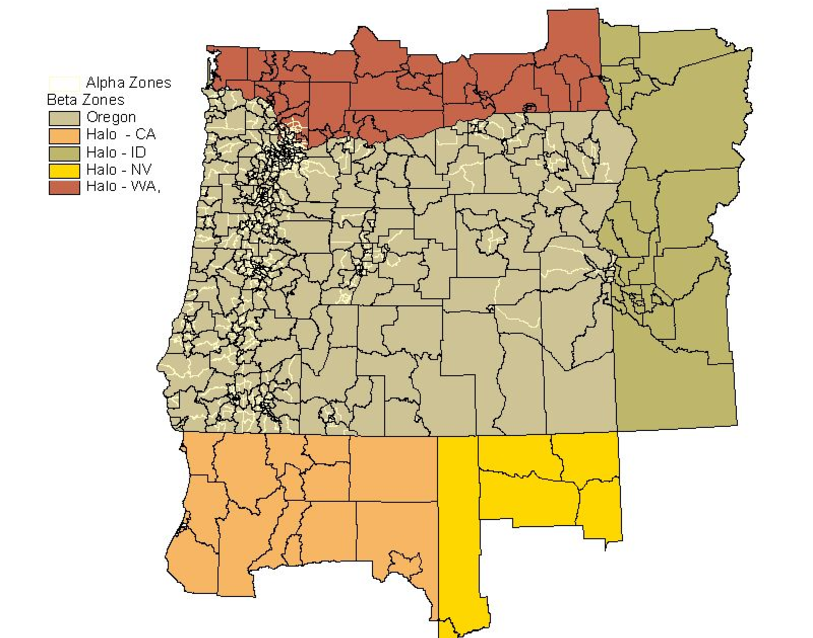
\includegraphics[scale=1.0]{overview/swim2-model-area}
\caption{SWIM2 modeled area zone system}\label{fig:swim2-model-area}
\end{figure}

\begin{table}
\centering
\caption{SWIM2 external stations}\label{tab:external-stations}
\begin{tabular}{cl|cl}
\hline
Alpha zone & External station & Alpha zone & External station \\
\hline
5001 & US101 (WA) & 5007 & I-84/US20 (ID) \\
\gray 5002 & I-5 (WA) & 5008 & US95 (NV, just north of I-80) \\
5003 & I-82 (WA) & 5009 & US395 (CA, just north of I-80) \\
\gray 5004 & US395/WA17 (WA) & 5010 & I-5 (CA) \\
5005 & US195 (WA) & 5011 & US101 (CA) \\
\gray 5006 & US95 (ID near WA border) & 5012 & Port of Portland Terminal 6 \\
\hline
\end{tabular}
\end{table}

\begin{figure}[!t]
\centering
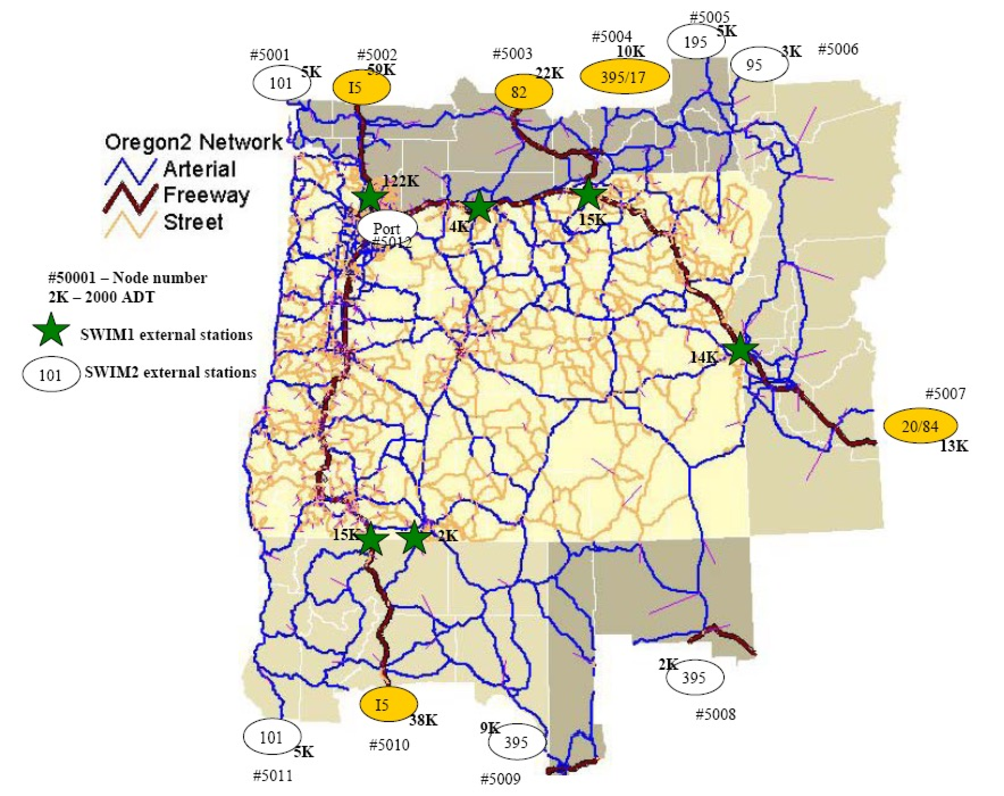
\includegraphics[width=6.25in]{overview/external-stations}
\caption{SWIM2 external stations}
\label{fig:swim2-external-stations}
\end{figure}
 
The activity allocation (AA) module operates on a more aggregated beta zone system (dark lines in Figure \ref{fig:swim2-model-area}), where the 12 external stations are replaced by six world markets listed in Table \ref{tab:world-markets}. There are 518 beta zones, collapsing zones only within Oregon, with a focus on the small urban zones. For example, the roughly 970 alpha zones in Portland are collapsed to approximate a set of 66 employment regions used by the Metro MPO model. In other urban areas, zones were collapsed based on a sliding population scale (approximately 25,000 persons per zone), respecting similar employment clusters and transportation commute sheds. In rural areas, homogenous public lands (e.g., BLM, National Forests) were collapsed, while retaining most county and all Area Commissions on Transportation (ACT) boundaries.\footnote{The ACTs are used in Oregon transportation planning, and provide a convenient way to divide the State into 12 areas.}

\begin{table}   % Table 2-2
\centering
\caption{AA world market zones and distance assumptions}
\label{tab:world-markets}
\begin{threeparttable}
\begin{tabular}{ccccl}
\hline
Zone & \multirow{2}{*}{Code} & Distance & External & \multirow{2}{*}{Definition} \\
number & & beyond halo\tnote{a} & station(s) & \\
\hline
6001 & N & 453/510 & 5002 & Washington and Canada \\
\gray6002 & NE & 453/510 & 5003, 5004 & Northern states of the Midwest \\
6003 & E & 1,661/1,399 & 5007 & Central and Eastern USA \\
\gray 6004 & S & 1,977/1,799 & 5010 & California, Southwestern states, Mexico \\
6005 & Ocean & 1500/600 & 5012 & Rest of the world\tnote{b} \\
\gray 6006 & Local & 75/75 & Non-Interstate & Local markets in neighboring states \\
\hline
\end{tabular}
\begin{tablenotes}
\footnotesize
\item[a] FHWA FAF3 distance data. Assumed 50 mph beyond halo to calculate equivalent travel time.
\item[b] Assumes \$600-900 import and \$700-2200 export costs to ship a Truck Equivalent Unit (TEU) between Portland and Japan (per May 2007 discussions with Port of Portland Staff). 
\end{tablenotes}
\end{threeparttable}
\end{table}

The six world markets defined in Table \ref{tab:world-markets} are only used only in the AA module. The direction of flow associated with them are shown in Figure \ref{fig:world-markets}, including the assumed distances to reach them beyond the model halo boundary. It is assumed that goods transported by truck and rail are limited to the US (except Hawaii), Canada, and Mexico. Imports and exports to other regions in the world are shipped by barge, either from the Port of Portland or other marine ports in the East or Southeastern regions of the USA. 

\begin{figure}   % Figure 2.3
\quote{\centering\small Note that the four directions shown refer to the directions N, NE, E, and S in\\Table \ref{tab:world-markets}. The shaded areas correspond to the areas each external market.\\}
\centering
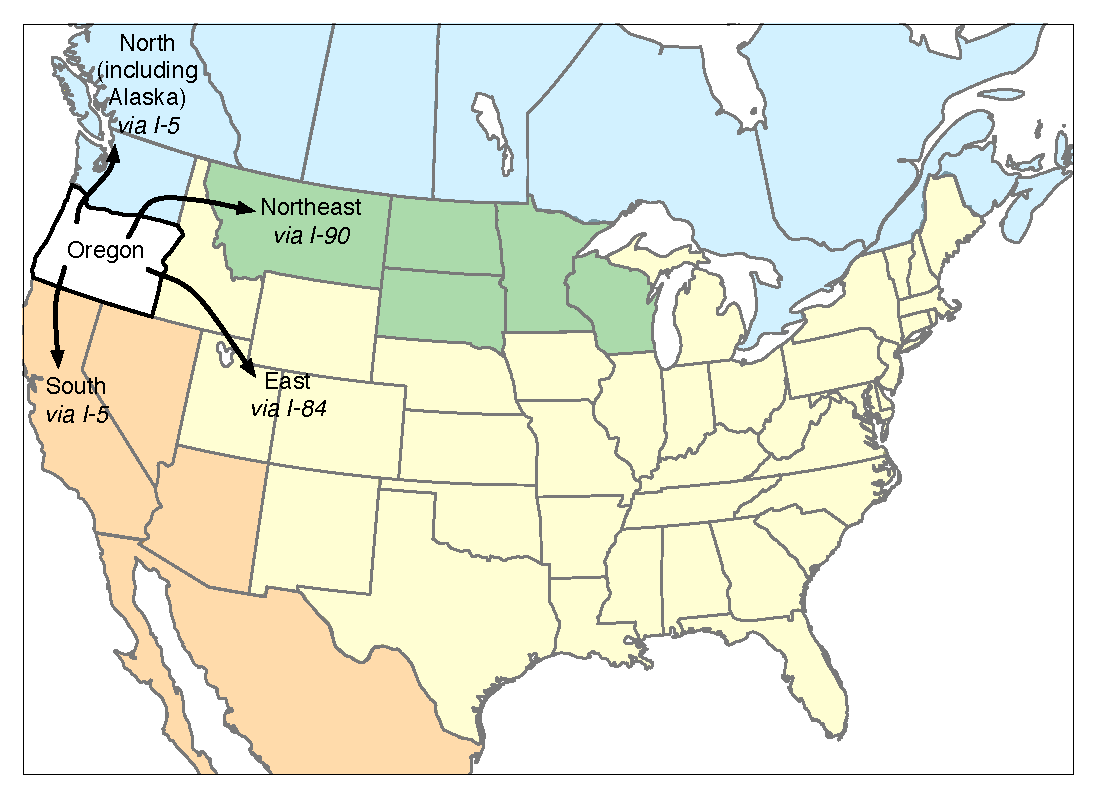
\includegraphics[width=5in]{overview/oregonregions}
\caption{Direction and extent of external and world markets in the SWIM2 system}
\label{fig:world-markets}
\end{figure}

The distances shown in Figure \ref{fig:world-markets} are based upon the Freight Analysis Framework (FAF)\footnote{\url{http://www.ops.fhwa.dot.gov/freight/freight_analysis/faf/}} Version 3.5 for truck flows and the truck portion of international intermodal flows. Data from the FAF base year of 2007 were used for these analyses. The approach described by \cite{moeckel10} was used for this purpose, assuming Euclidean distance between FAF zone centroids, with an additional distance added beyond the border in Canada (100 miles) and Mexico (300 miles). The distances within the model area, ranging from 90 to 425 miles (see Table 5 in \cite{moeckel10}), where excluded. In the case of the Oceanic market (zone 6005), an equivalent distance was identified that would result in the correct overall shipping costs, which varies by direction. The ``local'' world market (zone 6006) is assumed to support commodities that are traded within 75 miles of the model area.\footnote{The assignment of external origin/destination regions to external stations is based on a fastest travel time analysis to the centroids of each external region. An assumed average speed of 50 mph is used to calculate the equivalent travel time. World Market 6005 assumes an equivalent distance that allows accurate oceanic shipping costs, while using truck transport cost per mile as defined elsewhere in the AA module (CommoditiesI.csv). Oceanic time costs were assumed to be zero, as goods sent by ship tend to be less time-dependent. The air freight mode was ignored, as it represents less than one percent of all goods movement in Oregon, and at most two percent of any single commodity's flows.}

These six world markets link to the model transport network at the 12 external stations shown in Figure \ref{fig:swim2-external-stations} and Table \ref{tab:external-stations}. These external stations roughly parallel the likely rail as well as truck freight routes entering and leaving the model area. The local world market (zone 6006), trading within 75 miles of the model boundary, is linked to the minor roadway external stations, which consists of the non-Interstate highways shown in the Table.\footnote{Flows to and from World Market 6006 within 75 miles of the model border are currently not assigned, as they represent less than four percent of overall goods flows.}

% Figure 2.4 World Markets outside US (never referenced in the text, so omitted)

The aggregate land development (ALD) component uses a 15-region aggregation of the alpha zones for making land development decisions. These regions, shown in Figure \ref{fig:ald-regions}, represent SWIM2 land development markets within the study area.

\begin{figure}[!t]
\centering
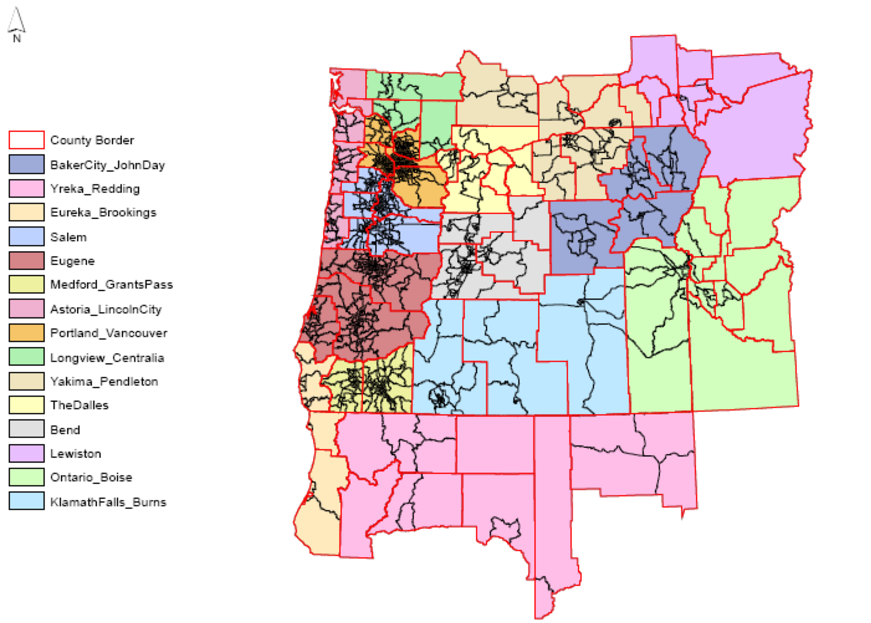
\includegraphics[width=6.25in]{overview/ald-regions}
\caption{Aggregate land development (ALD) regions}
\label{fig:ald-regions}
\end{figure}

\subsection{Category definitions}\label{sec:category-definitions}
At its core the SWIM2 system encapsulates a spatial input-output (IO) formulation that resides in the AA component. A summary of the IO make and use table framework and the categories of activities and commodities used within them is shown in Figure \ref{fig:make-use-summary}. The Figure shows the specific types of economic interactions represented in the model. Commodity production is represented in the make table at the top of the Figure. Commodity consumption is represented in the use table at the bottom of the Figure. Commodities flow down the columns from where they are produced to where they are consumed. The general nature of the exchange location for each commodity category and the treatment of imports and exports are also indicated.

The industry, government and household activity categories used in SWIM2 are shown in Tables \ref{tab:activity-industry} and \ref{tab:size-income}. Certain industries have been allowed to use more than one space type, exploiting new AA routines that calculate zonal size terms based on quantities of space, and so is better able to allocate activities in zones with limited space-type availability. Some activities are classified based upon the North American Industrial Classification System (NAICS)\footnote{\url{http://www.census.gov/eos/www/naics/}}, while others are grouped together to define land use, transport, or labor markets (e.g., Services-At Customers Business, Services-Storefront). In general, a given industrial sector is split into blue-collar and white-collar (or ``office support'') components using associated production and office space categories, respectively. In this way the allocation processes in the AA component can consider the very different location behavior and space requirements of these two categories. Internal office support activities strictly produce management services consumed by their corresponding industries. For instance, Services at customer's house are self-employed workers who sell their services to households (e.g., housekeepers, nannies, handymen).

\begin{sidewaysfigure}     % Figure 2-6
\centering
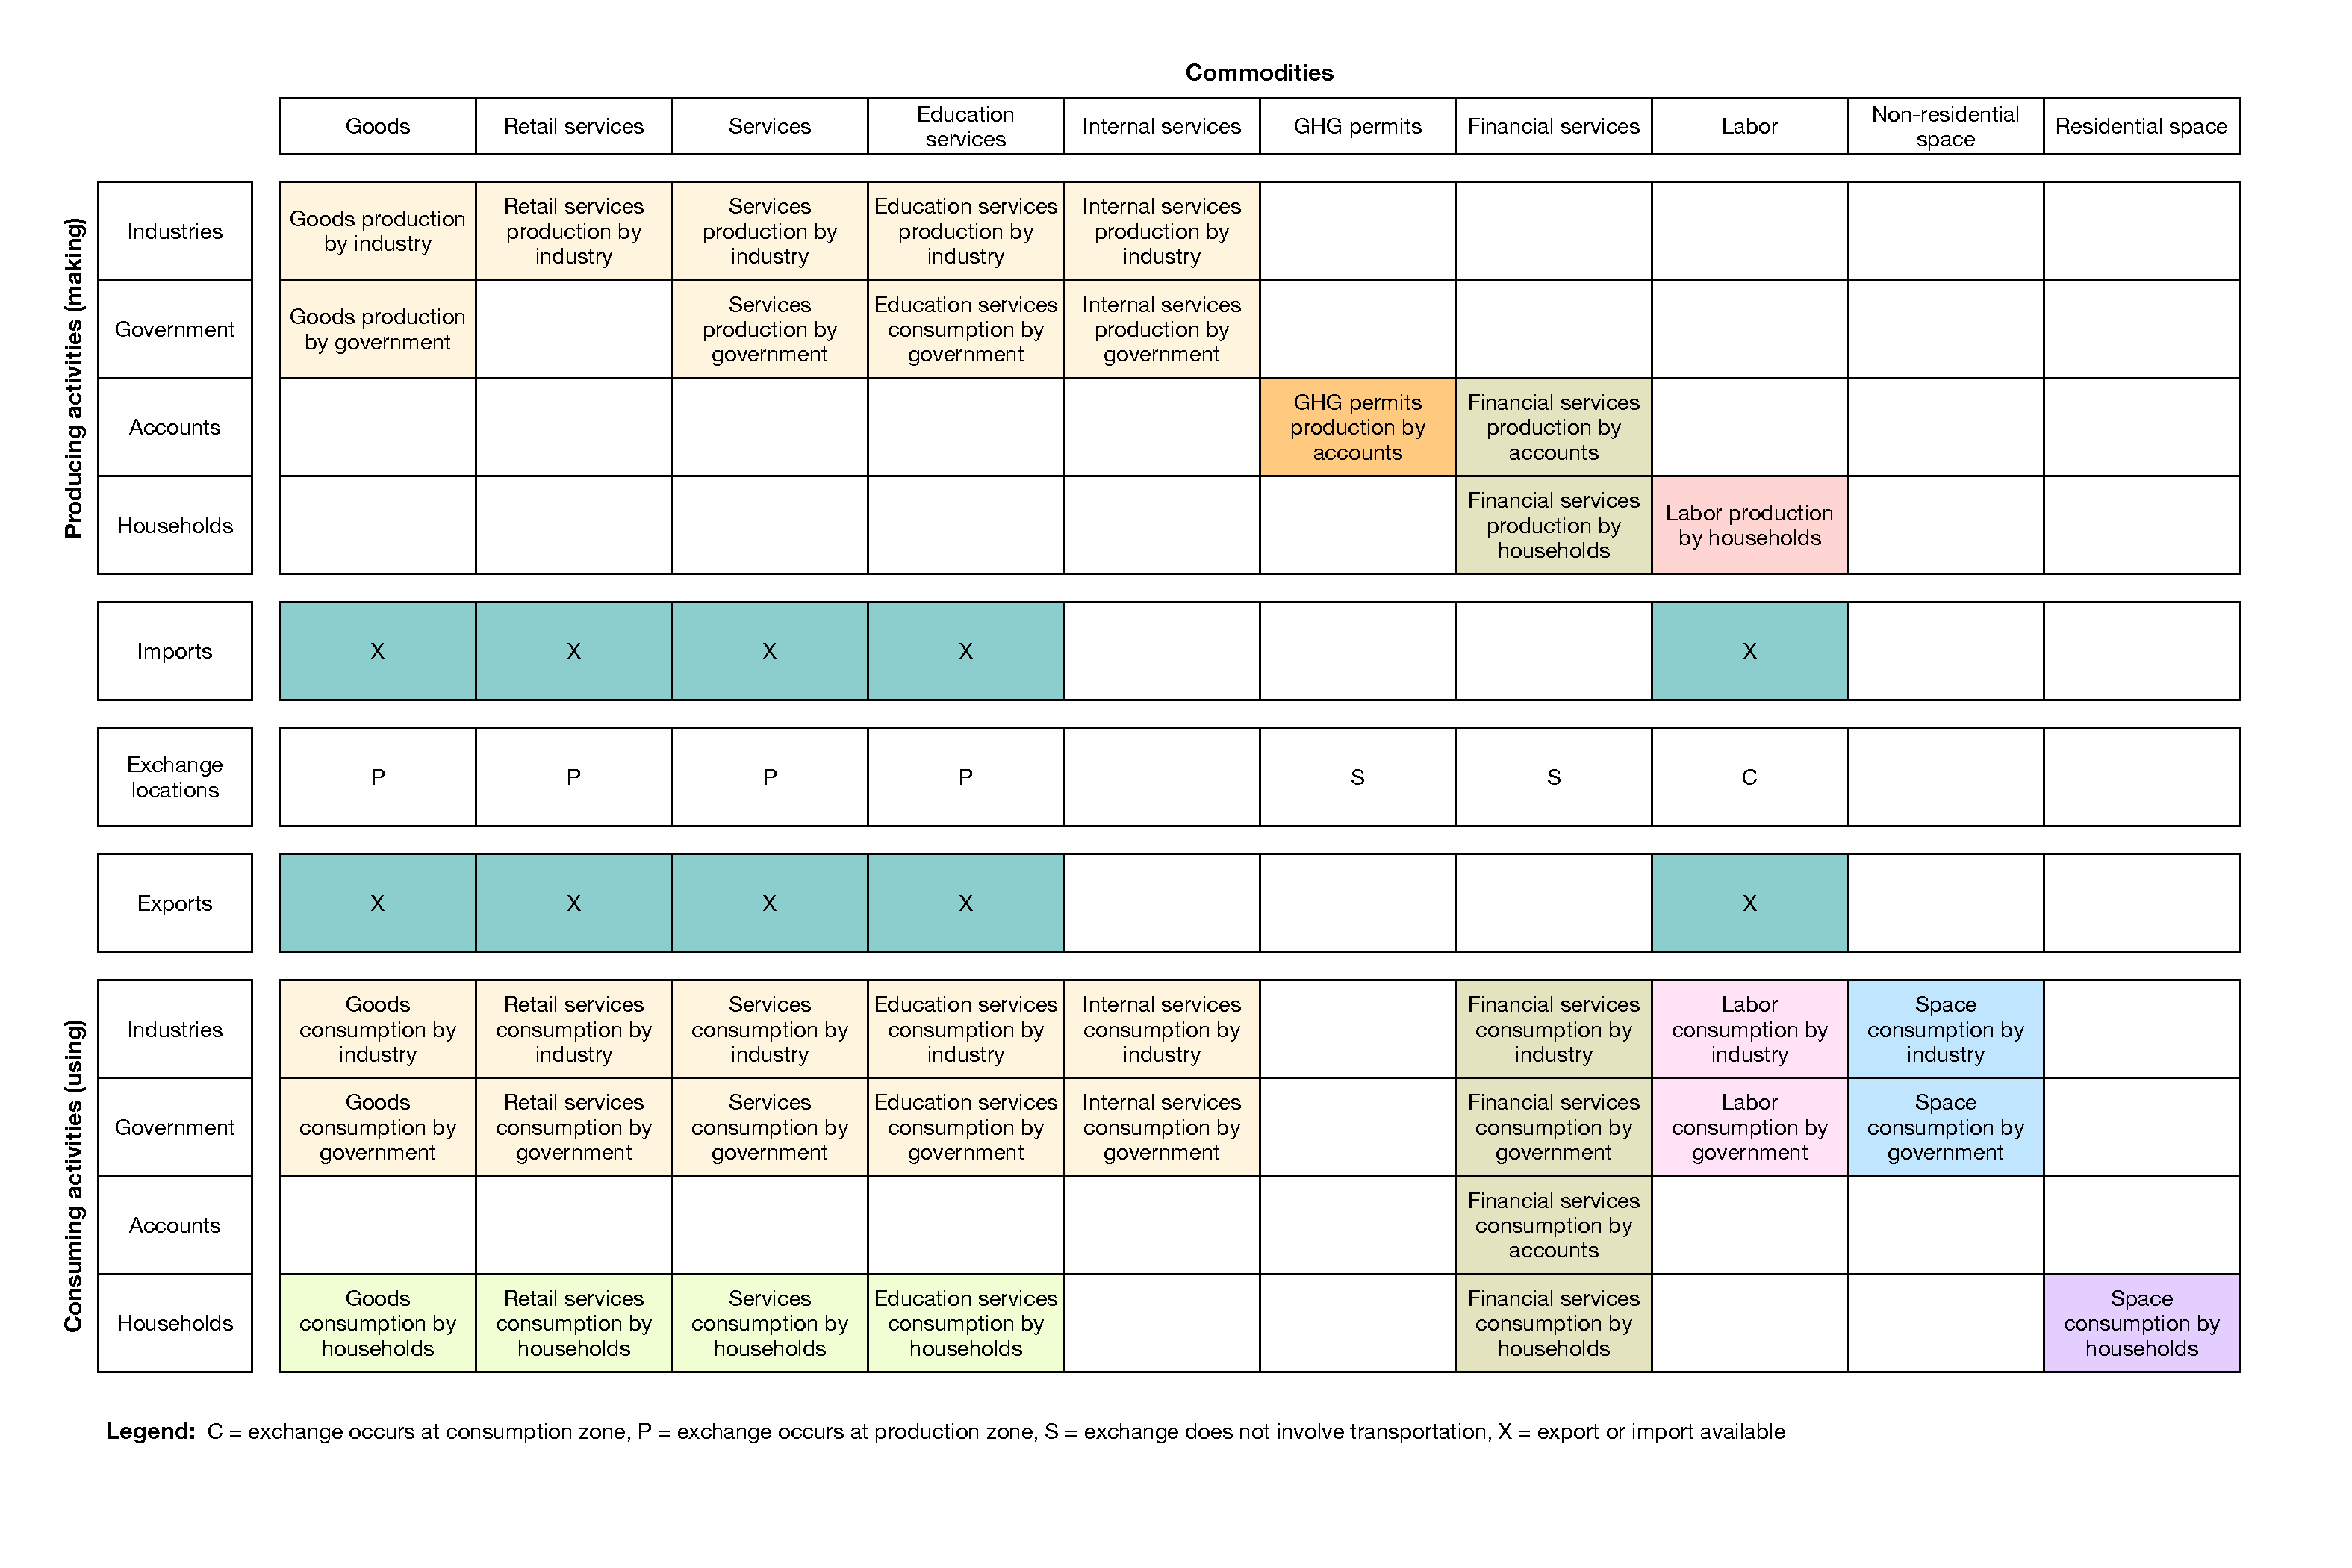
\includegraphics[scale=0.45]{overview/make-use-summary}
\caption{Summary of commodities made and used by various activities within the model}
\label{fig:make-use-summary}
\end{sidewaysfigure}

% Table 2-3 in v29
\begin{table}
\centering
\caption{Activities by industry}\label{tab:activity-industry}
\fontsize{9.5}{10.5}\rm
\begin{tabular}{|l|l|l|}
\hline
Industry                        & Floorspace options & Internal services \\
\hline
Resource-Ag and Mining          & FLR Agriculture & Internal Services Resources \\
Resource-Forest                 & FLR Logging & Internal Services Resources \\
Resource Office Support         & FLR Office & \\
\hline 	
Energy-Electric                 & FLR Heavy Industry & Internal Services Energy \\
Energy-Natural Gas              & FLR Heavy Industry & Internal Services Energy \\
Energy-Petroleum                & FLR Heavy Industry & Internal Services Energy \\
Energy Office Support           & FLR Office &  \\
\hline
Utilities-Other                 & FLR Office, FLR Light Industry & Internal Services Utilities \\
Utilities-Other Office Support  & FLR Office &  \\
\hline
Construction-Maintenance        & n/a & Internal Services Construction \\
Construction-Nonresidential     & n/a & Internal Services Construction \\
Construction-Other              & n/a & Internal Services Construction \\
Construction-Residential        & n/a & Internal Services Construction \\
Construction Office Support     & n/a & \\
\hline
Manufacturing-Food HI           & FLR Heavy Industry & Internal Services Manufacturing \\
Manufacturing-Food LI           & FLR Light Industry & Internal Services Manufacturing \\
Manufacturing-High Tech HI      & FLR Heavy Industry & Internal Services Manufacturing \\
Manufacturing-High Tech LI      & FLR Light Industry & Internal Services Manufacturing \\
Manufacturing-High VTW HI       & FLR Heavy Industry & Internal Services Manufacturing \\
Manufacturing-High VTW LI       & FLR Light Industry & Internal Services Manufacturing \\
Manufacturing-Low VTW HI        & FLR Heavy Industry & Internal Services Manufacturing \\
Manufacturing-Wood and Paper HI & FLR Heavy Industry & Internal Services Manufacturing \\
Manufacturing Office Support    & FLR Office & \\
\hline
Information                     & FLR Office & Internal Services Information \\
Information Office Support      & FLR Office, FLR Light Industry & \\
\hline
Wholesale                       & FLR Warehouse & Internal Services Wholesale \\
Wholesale Office Support        & FLR Office & \\
\hline
Transport                       & FLR Warehouse & Internal Services Transport \\
Transport Office Support        & FLR Office &  \\
\hline
Retail-Automotive               & FLR Retail &  \\
Retail-Store                    & FLR Retail & Internal Services Retail Store \\
Retail-Store Office Support     & FLR Office &  \\
Retail-Nonstore                 & FLR Office &  \\
\hline
Finance and Insurance           & FLR Office &  \\
Real Estate                     & FLR Office &  \\
\hline
Entertainment                   & FLR Retail &  \\
Accommodations                  & FLR Accommodation &  \\
Eating and Drinking Places      & FLR Retail, FLR Accommodation &  \\
Services-Professional and Technical & FLR Office &  \\
Services-at Customer's Business & FLR Light Industry &  \\
Services-at Customer's House    & n/a &  \\
Services-Business               & FLR Office &  \\
Services-Nonprofit              & FLR Office, FLR Institutional &  \\
Services-Storefront             & FLR Retail &  \\
\hline
Health-Hospital                 & FLR Hospital &  \\
Health-Care Facility            & FLR Institutional &  \\
Health-Other                    & FLR Office, FLR Light Industry &  \\
\hline
Education-K12                   & FLR K12 & Internal Services Education K12 \\
Education-K12 Office Support    & FLR Office &  \\
Education-Higher                & FLR Office, FLR Institutional &  \\
\hline
Government Administration Operations & n/a & Internal Services GovAdmin \\
Government Administration Office Support & n/a &  \\
\hline
\end{tabular}
\end{table}    % Table 2.3
% Table 2-4 in v29
\begin{table}
\centering
\caption{Household size and income categories (2009 dollars)}\label{tab:size-income}
\fontsize{11.0}{13.75}\rm
\begin{tabular}{lcl}
\hline
Code & Household income & Household size \\
\hline
HH0to8k1to2 & \$0 to 7,999 & 1 to 2 persons \\
\gray HH0to8k3plus & \$0 to 7,999 & 3 or more persons \\
HH8to15k1to2 & \$8,000 to 14,999 & 1 to 2 persons \\
\gray HH8to15k3plus & \$8,000 to 14,999 & 3 or more persons \\
HH15to23k1to2 & \$15,000 to 22,999 & 1 to 2 persons \\
\gray HH15to23k3plus & \$15,000 to 22,999 & 3 or more persons \\
HH23to32k1to2 & \$23,000 to 31,999 & 1 to 2 persons \\
\gray HH23to32k3plus & \$23,000 to 31,999 & 3 or more persons \\
HH32to46k1to2 & \$32,000 to 45,999 & 1 to 2 persons \\
\gray HH32to46k3plus & \$32,000 to 45,999 & 3 or more persons \\
HH46to61k1to2 & \$46,000 to 60,999 & 1 to 2 persons \\
\gray HH46to61k3plus & \$46,000 to 60,999 & 3 or more persons \\
HH61to76k1to2 & \$61,000 to 75,999 & 1 to 2 persons \\
\gray HH61to76k3plus & \$61,000 to 75,999 & 3 or more persons \\
HH76to106k1to2 & \$76,000 to 105,999 & 1 to 2 persons \\
\gray HH76to106k3plus & \$76,000 to 105,999 & 3 or more persons \\
HH106kUp1to2 & \$106,000 and over & 1 to 2 persons \\
\gray HH106kUp3plus & \$106,000 and over & 3 or more persons \\
\hline
\end{tabular}
\end{table}      % Table 2.4

Other considerations in the classification of industries include:
\begin{itemize}
\item The distributors and generators of energy used in buildings (natural gas distribution, electrical power generation transmission and distribution, and petroleum) were separated into three subcategories to support better representation of energy use and associated greenhouse gas emissions. Construction was divided into residential buildings, non-residential buildings, maintenance, other buildings and office support, to better support the ALD component.
\item Food, wood and paper, and high technology remain as separate manufacturing sectors but, were divided into heavy industry and light industry. The remaining manufacturing sectors were divided based on the value-to-weight ratio of their production, to separate those dependent on the movement of heavy goods in large trucks and by rail. They were also split into heavy and light industry categories.
\item Wholesale and retail are two separate categories. The first one was split into Wholesale and Wholesale Office Support. The retail category was split into four subcategories: Automotive, Store, Store Office Support and Non-store.
\item Transportation, Information, and Utilities are three separate categories. Each of them was split into two in order to represent the management of the service, using a subcategory of Office Support.
\item Finance and Insurance, and Real Estate remain as separate categories.
\item Health as category includes three subcategories: Hospitals, Care Facility and Other.
\item Three subcategories can be found in Education: Education-K12 (previously called Grade-school), Education Office Support and Higher Education.
\item Entertainment, Accommodations and Eating and Drinking places are separate sector industries.
\item Services as a sector industry was split based on two criteria: the space type they use and the NAICS two-digit industry categories. In the first group are three subcategories: Services-At Customer's Business, Services-At Customer's House, and Services-Storefront. In the second group are: Services-Professional and Technical, Services-Business and Services-Non-profit.
\item For government administration category two subcategories were set-up: Operations and Office Support.
\end{itemize} 

Household activities were classified as categories of household income and size (persons per household) based on the original 1990 Census definitions, inflated to 2009 dollars using prices index for gross domestic product (GDP) from the Bureau of Economic Analysis (BEA) of the U.S. Department of Commerce. Household activities include the production of labor and consumption of various goods (primarily through retail) and services. Household income groups reflect the original SWIM2 1990 Census categories, with income amounts inflated to 2009 dollars (consistent with the 2010 census and 2009 IMPLAN) using a 1.52 GDP deflator.

Group quarters (GQ) are represented in SWIM2 using the same definitions used in the 2005-09 American Community Survey (ACS)\footnote{\url{http://www.census.gov/acs/www/}}. They represent six percent of all Oregon households, evenly split between institutional and non-institutional (e.g., student) populations. In a summary of the 2009 ACS PUMS it was found that half of the GQ residents are in institutions. The other half, which includes students, consists mainly of 1--2 person multi-family households.

The commodities produced and consumed in the model, including study area imports and exports, are shown in Table \ref{tab:goods-categories}. Industry and government activities include the production and consumption of goods and services. The commodities shown in the Table are tracked in the AA and commercial travel (CT) components, including 39 types of goods based on the Standard Classification of Transportable Goods (SCTG) categories\footnote{\url{https://www.census.gov/svsd/www/cfsdat/cfs071200.pdf}}. Energy flows, to include natural gas and electricity, were added so that their levels could be tracked. However, since these energy sources are not transported by truck they are not explicitly addressed in the CT module. In addition, within AA two commodities are combined in order to eliminate small and problematic tobacco (SCTG 9) shipments and to avoid splitting the sand and gravel industries (SCTG 11 and 13). The full set of SCTG file outputs will still be produced by AA, but one will have zero flows. This enables their explicit treatment within AA without accompanying changes in the CT module.

\begin{table}   % Table 2-6
\centering
\caption{Commodities---goods categories}\label{tab:goods-categories}
\small
\begin{tabular}{ll}
\hline
SCTG code & Description \\
\hline
SCTG1\_FKP\_L VSK & Live Animals and Fish \\
\gray SCTG2\_FKP\_AGRI\_cereal & Cereal Grains (including seed) \\
SCTG3\_FKP\_AGRI\_other & Other Agricultural Products, except for Animal Feed \\
\gray SCTG4\_FKP\_FEED & *Animal Feed and Products of Animal Origin, n.e.c. \\
SCTG5\_FKP\_FOOD\_meat & *Meat, Fish, and Seafood, and Their Preparations \\
\gray SCTG6\_FKP\_AGRI\_grain & *Milled Grain Products and Preparations, and Bakery Products \\
SCTG7\_FKP\_FOOD\_prep & *Other Prepared Foodstuffs, and Fats and Oils \\
\gray SCTG8\_FKP\_FOOD\_alc & *Alcoholic Beverages \\
SCTG9\_FKP\_FOOD\_tob & Tobacco Products \\
\gray SCTG10\_CMS\_CLAY & Monumental or Building Stone \\
SCTG11\_CMS\_SAND & Natural Sands \\
\gray SCTG12\_CMS\_STON & Gravel and Crushed Stone \\
SCTG13\_CMS\_MINE\_nonmet & Non-Metallic Minerals, n.e.c. \\
\gray SCTG14\_CMS\_MINE\_met & Metallic Ores and Concentrates \\
SCTG15\_PCC\_COAL & Coal \\
\gray SCTG16\_PCC\_PETR\_crude & Crude Petroleum Oil \\
SCTG17\_PCC\_FUEL & *Gasoline and Aviation Turbine Fuel \\
\gray SCTG18\_PCC\_PETR\_oil & *Fuel Oils \\
SCTG19\_PCC\_COAL\_prod & Coal and Petroleum Products, n.e.c. \\
\gray SCTG20\_PCC\_CHEM\_basic & Basic Chemicals \\
SCTG21\_PCC\_CHEM\_pharma & *Pharmaceutical Products \\
\gray SCTG22\_PCC\_CHEM\_fert & Fertilizers \\
SCTG23\_PCC\_CHEM\_prod & *Chemical Products and Preparations, n.e.c. \\
\gray SCTG24\_PCC\_PETR\_plast & Plastics and Rubber \\
SCTG25\_FWP\_LOGS & Logs and Other Wood in the Rough \\
\gray SCTG26\_FWP\_WOOD & Wood Products \\
SCTG27\_PPP\_P APR\_puplp & Pulp, Newsprint, Paper, and Paperboard \\
\gray SCTG28\_PPP\_P APR\_paper & Paper or Paperboard Articles \\
SCTG29\_PPP\_P APR\_print & *Printed Products \\
\gray SCTG30\_OTH\_CLTH & *Textiles, Leather, and Articles of Textiles or Leather \\
SCTG31\_CMS\_MIN & Non-Metallic Mineral Products \\
\gray SCTG32\_MIT\_METL\_base & Base metal in primary or semi-finished forms and in finished basic shapes  \\
SCTG33\_MIT\_METL\_prod & Articles of Base Metal \\
\gray SCTG34\_MIT\_MACH & Machinery \\
SCTG35\_MIT\_ELCT & Electronic, electrical, and office equipment and components \\
\gray SCTG36\_MIT\_TRAN & *Motorized and Other Vehicles (including parts) \\
SCTG37\_MIT\_INST\_transp & Transportation Equipment, n.e.c. \\
\gray SCTG38\_MIT\_INST\_prec & Precision Instruments and Apparatus \\
SCTG39\_OTH\_FURN & *Furniture and fixtures and lighting and illuminated signs \\
\gray SCTG40\_OTH\_MISC & *Miscellaneous Manufactured Products \\
SCTG41\_WASTE\_SCRAP & Waste and Scrap \\
\hline
\end{tabular}
\end{table}

The services tracked in the AA and person travel (PT) modules are shown in Table \ref{tab:service-categories}. Internal services, defined as ``value-added office labor,'' spatially connect the production and office components of split industries. This commodity is the service provided by management and other office support workers to the production floor of the same industry. In many cases, this flow represents a relationship between two establishments of the same firm.

% Table 2-5 in v29
\begin{table}
\centering
\caption{Commodities and service categories}\label{tab:service-categories}
\fontsize{11.5}{14.375}\rm
\begin{tabular}{|l|l|}
\hline
Services category & Services included \\
\hline
Retail Services (p) & Retail Trade \\
\hline
Services & Energy (c) \\
 & Transport (p) \\
 & Wholesale Trade (p) \\
 & Construction (c) \\
 & Communications and Utilities (p) \\
 & Accommodations (p) \\
 & Personal and Other Services and Amusements (p) \\
 & Entertainment Services (p) \\
 & Food Services (p) \\
 & Health Services (p) \\
 & FIRE, Business, and Professional services (c) \\
 & Government Administration (p) \\
\hline
Education Services (p) & Teaching K12 \\
 & Higher Education \\
\hline
Environmental (s) & GHG Permits \\
\hline
Financial Services (s) & Government Support Receipts \\
 & Tax Receipts \\
 & Investing Receipts \\
 & Proprietor Income Receipts \\
 & Return Investment Receipts \\
 & Capital Transfer Receipts \\
 & Education Reports to Sponsors \\
\hline
Internal Services (c) & Internal Services Resources \\
 & Internal Services Energy \\
 & Internal Services Construction \\
 & Internal Services Manufacturing \\
 & Internal Services Wholesale \\
 & Internal Services Retail Store \\
 & Internal Services Transport \\
 & Internal Services Information \\
 & Internal Services Utilities \\
 & Internal Services Education K12 \\
 & Internal Services Government Administration \\
\hline
\end{tabular}
\end{table}  % Used to be Table 2-5, but mis-numbered because of duplicate Tables 2-6

Labor is included as a commodity that is produced by households and consumed by economic production activities. As such, the synthetic population generator (SPG) respects the home end while PT respects the work end of labor flows produced by the AA component. Different labor occupation categories from 2000 Standard Occupational Categories (SOC)\footnote{\url{http://www.bls.gov/soc/}} codes are treated as different commodity categories. Thirteen categories of labor have been defined considering occupations and years of education, as shown in Figure \ref{fig:labor-occupation-categories}. The new labor categorization is based on the following three principles:
\begin{itemize}
\item Four groups of two-digit SOC codes, for comparing with any data sources that summarize employment based on 2-digit SOC.
\item Within three of the four groups, the occupations requiring lower education (based on observed education levels in the ACS PUMS) were grouped together, with the idea that these workers would have a lower income, a lower value of time, and could more easily and more readily switch between two-digit SOC categories. These were named ``unskilled'' occupations, although of course in every occupation there are some highly skilled individuals.
\item Within the higher education occupations, occupations were further split into more detailed two-digit SOC groups.
\end{itemize}

\begin{figure}[!t]   % A figure that was labeled as one of several Tables 2-5
\centering
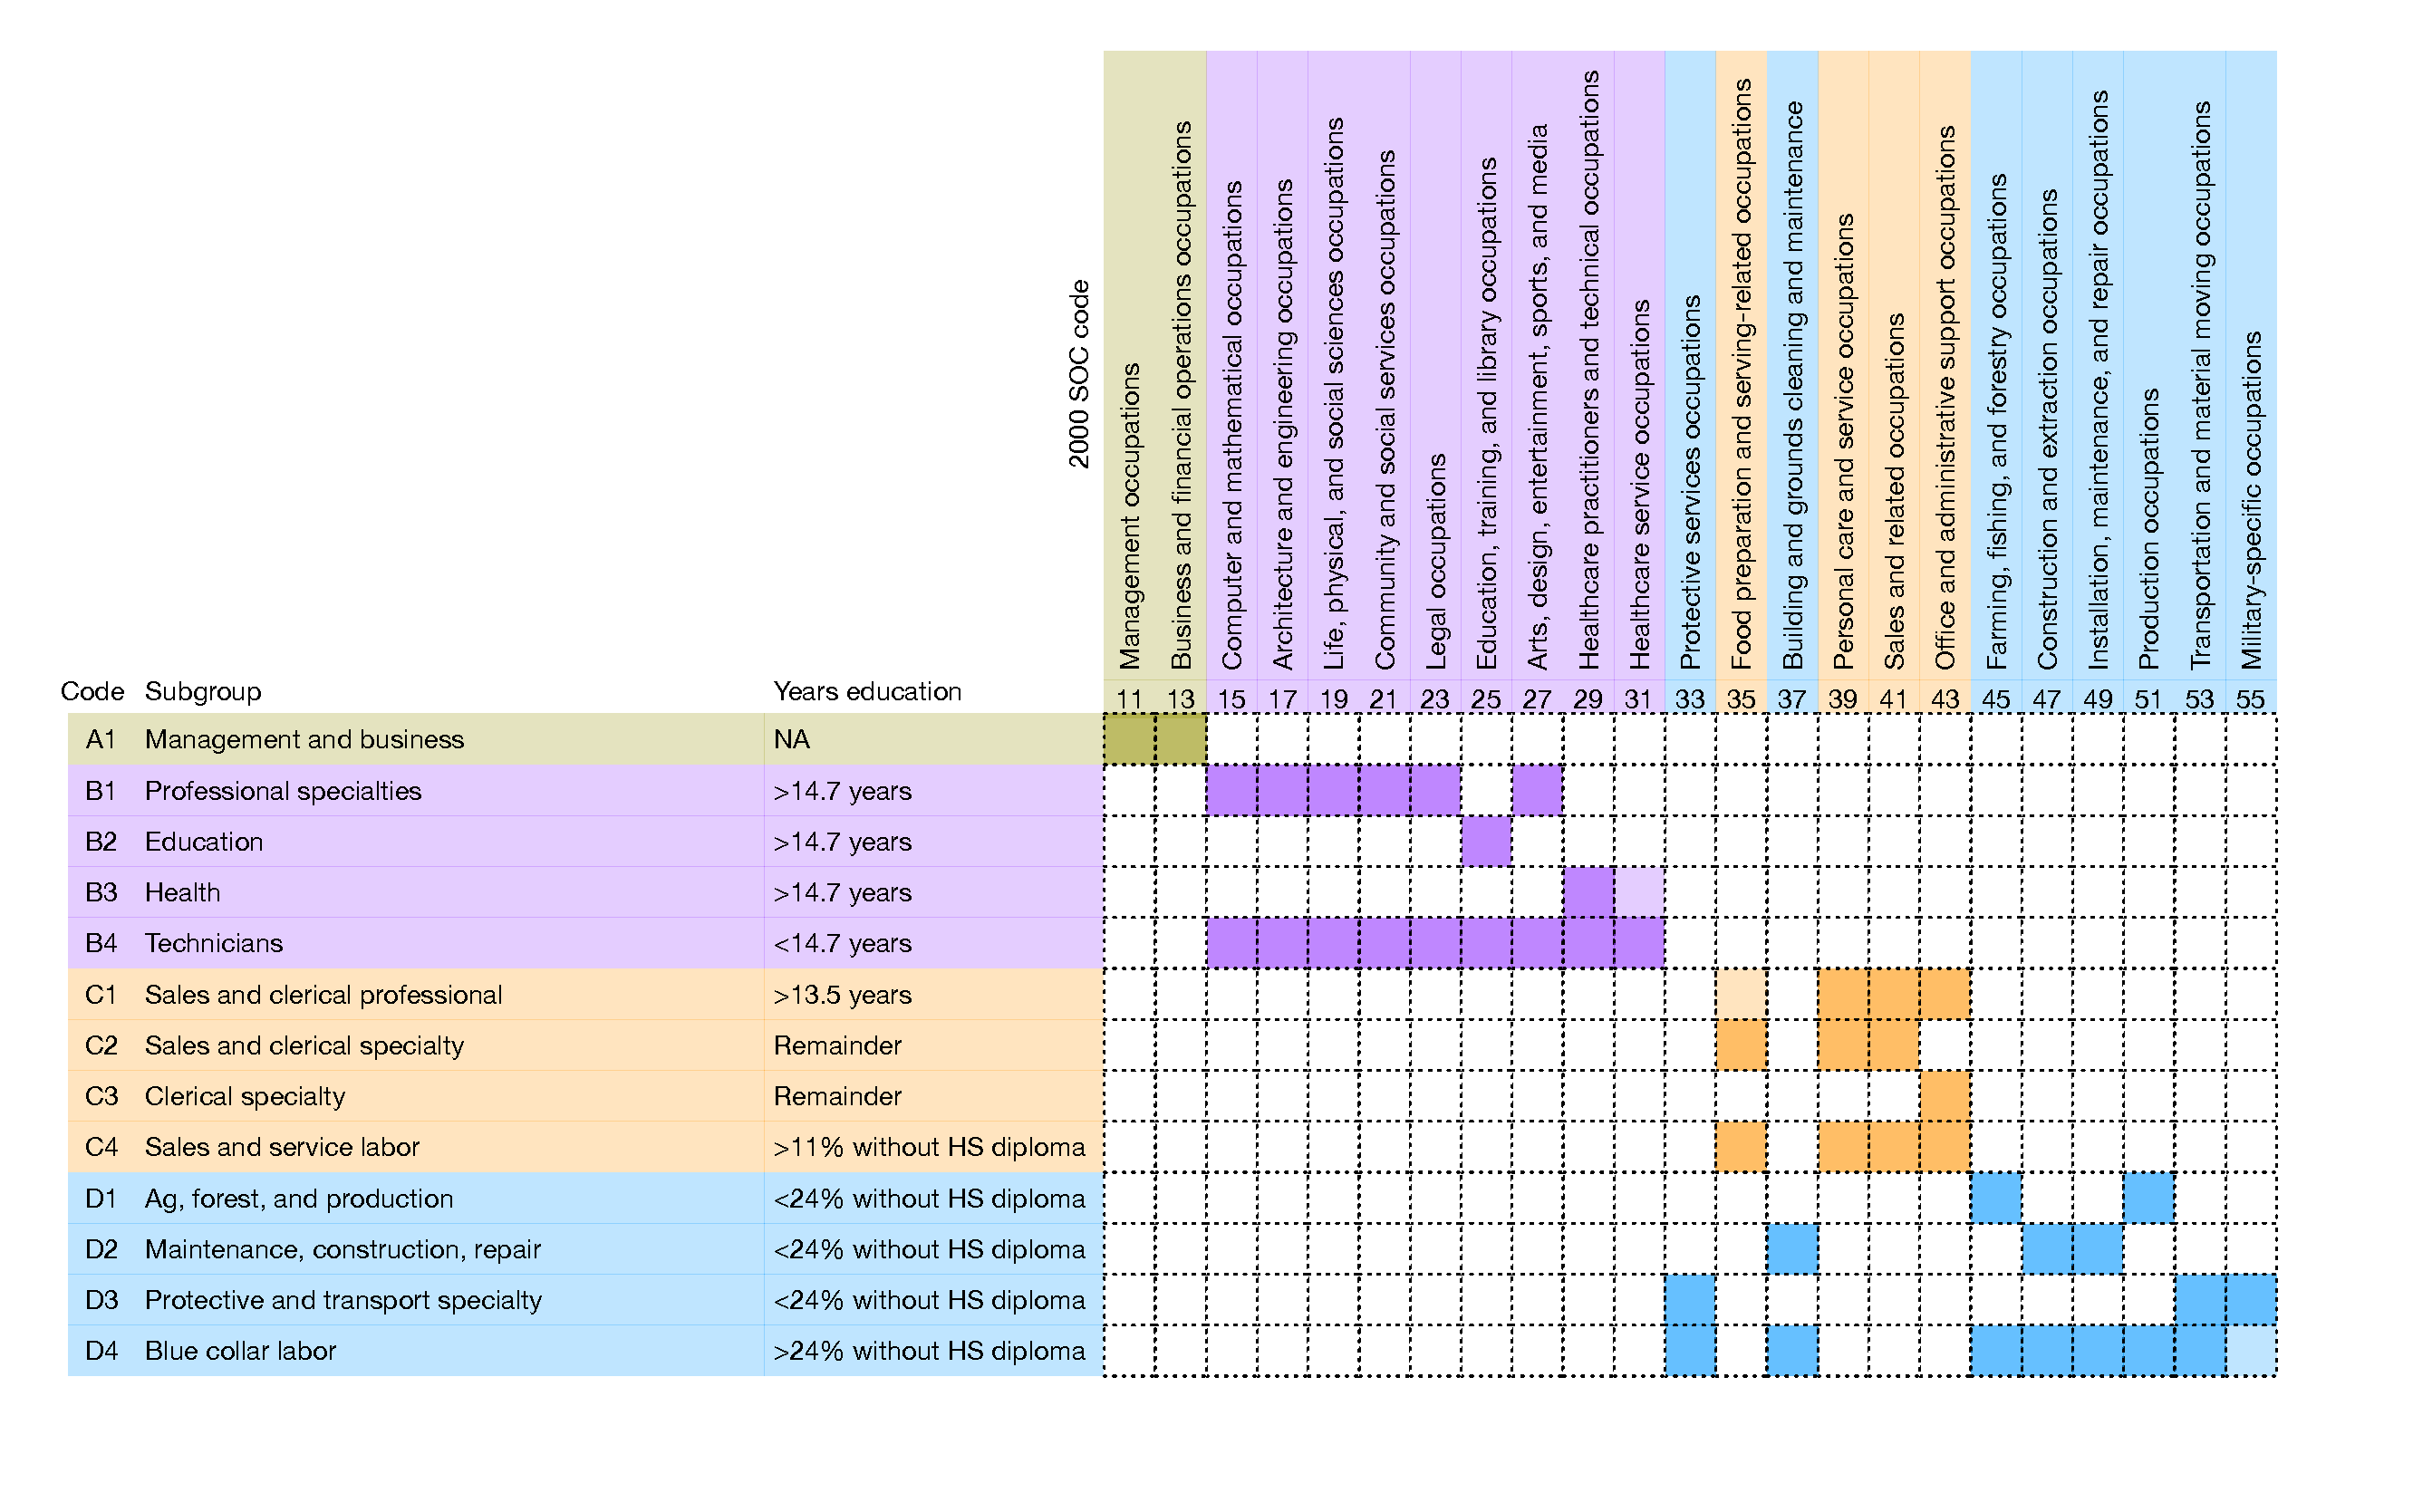
\includegraphics[scale=0.4, trim=11mm 23mm 0mm 0mm, clip]{overview/commodities-labor-categories}  % trim=l b r t
\caption{Labor occupation categories}\label{fig:labor-occupation-categories}
\end{figure}

Floorspace categories are shown in Table \ref{tab:floorspace-categories}, while Table \ref{tab:activity-industry} identifies which floorspace types are used by each industry category. ALD adjusts the inventory of developed floorspace available in alpha zones in each model period. The original FLR\_Depot space type was ambiguous, and has been combined with FLR\_Warehouse. Additionally, heavy and light industry spaces definitions have been updated slightly. Likely more light industry will be demanded, but is expected to be within the tolerance of ALD's current interpretation of zoning inputs.   

% Table 2-6 in v29
\begin{table}
\centering
\caption{Floorspace categories}\label{tab:floorspace-categories}
\fontsize{11.0}{13.75}\rm
\begin{tabular}{|l|l|l|}
\hline
Residential floorspace & Non-residential floorspace & Resource floorspace \\
\hline
FLR SFD (Single Family Home) & FLR Hospital & FLR Agriculture (includes Mining) \\
FLR AT (Attached Home) & FLR Retail & FLR Logging \\
FLR MH (Manufactured Home) & FLR Office & \\
FLR RRMH (Rural Residential MH) & FLR Heavy Industry & \\
FLR RRSFD (Rual Residential SFD) & FLR Light Industry & \\
FLR MF (Multi-family, Institutional) & FLR Warehouse & \\
 & FLR Institutional &  \\
 & FLR Accommodation & \\
 & FLR Government Support & \\
 & FLR K12 (Grade School) & \\
\hline
\end{tabular}
\end{table}   % Table 2-6

The various modes and vehicles used in the model to transport person and goods flows are shown in Table \ref{tab:transport-modes}. Non-motorized passenger modes and non-truck freight modes are not assigned to the network.

\begin{sidewaystable}
\centering
\caption{Transport modes and vehicle types}\label{tab:transport-modes}
\begin{tabular}{|l|l|l|l|c|}
\hline
Type & Code & Trip mode & Definition & Component(s) \\
\hline
Person & DA & Drive alone & Single-occupant auto & SDT, LDT \\
\gray \cellcolor{white}travel & SR2 & Shared ride 2 & Two-occupant auto & SDT, LDT \\
 & SR3P & Shared ride 3+ & Three or more occupant auto & SDT, LDT \\
\gray \cellcolor{white}& WALK & Walk & Walk & SDT \\
 & BIKE & Bicycle & Bicycle & SDT \\
\gray \cellcolor{white}& SCHOOL\_BUS & School bus & School bus (not assigned) & SDT \\
 & TRANSIT\_WALK & Walk to transit & Walk-access transit & LDT \\
\gray \cellcolor{white}& TRANSIT\_DRIVE & Drive to transit & Drive-access transit & LDT \\
 & AIR & Drive to air & Drive-access air travel within modeled area & LDT \\
\gray \cellcolor{white}& HSR\_DRIVE & Drive to HSR & Drive-access intercity rail & LDT \\
 & HSR\_WALK & Walk to HSR & Walk-access to intercity rail & LDT \\
\hline
\gray \cellcolor{white}Freight & TRK1 & Truck type 1 & $<$34,000 lbs. (likely single-unit) & CT, ET \\
 & TRK2 & Truck type 2 & 34,000--64,000 lbs. & CT, ET \\
\gray \cellcolor{white}& TRK3 & Truck type 3 & 64,000--80,000 lbs. (articulated) & CT, ET \\
 & TRK4 & Truck type 4 & 80,000--105,500 lbs. (articulated) & CT, ET \\
\gray \cellcolor{white}& TRK5 & Truck type 5 & $>$105,500 lbs. (articulated) & CT, ET \\
 & SAA & Air freight & Air freight (not assigned) & \\
\gray \cellcolor{white}& SRR & Rail freight & Rail freight (not assigned) & \\
 & SWA & Waterborne freight & Waterborne freight (not assigned) & \\
\gray \cellcolor{white}& SPA & Pipeline & Pipeline freight (not assigned) & \\
\hline
\end{tabular}
\end{sidewaystable}  % Table 2-7
 
The attributes of persons and households created in the SPG module and used in the PT module are shown in Figure \ref{fig:synthetic-attributes}. The Table also shows the 1990 Census-based coding categories for each attribute. The fields of the synthetic population used in the SWIM2 model are described below, with synthesized value marked by asterisk. The others are retained from the drawn PUMS record. SPG controls only for workers per household, worker industry, and person age. SWIM2 assigns home location and work location based on AA labor flows:
\begin{itemize}
\item \textit{Household-Person File Link (HH\_ID, PER\_ID):} The household attributes were linked to each person in the household, by storing a household (HH\_ID) and person (PER\_ID) ID in the person file. HH\_ID are numbered sequentially across the whole sample, starting with 1. PER\_IDs are numbered sequentially across all persons in a household. 
\item \textit{Household Attributes (PERSONS, AUTOS*):} The number of persons and the total number of autos in the household. The Census auto value is updated by the PT module.
\item \textit{Home Location (AZONE):} The alpha zone location of the household, assigned by SPG2, consistent with AA labor flows by occupation. 
\item \textit{Household Income (RHHINC):} Total household income in units of 2009 dollars.
\item \textit{Residential Floorspace Type (UNITS1, SINGLE\_FAMILY*):} The household's residential floor\-space type is indicated by the number of units in the dwelling unit (UNITS1). In PT, a binary variable is created to indicate whether the dwelling unit is a single family unit. 
\item \textit{Demographics (AGE, SEX):} Age and gender for each household member.
\item \textit{Employment Information (RLABOR, OCCUP, INDUSTRY, ESR*, SW\_OCC*, SW\_SPLIT\_IND*, WORKTAZ*):} Employment status for each household member indicates whether each person is employed or not in the labor force (RLABOR). If employed, PUMS occupation and industry from PUMS (OCCUP, INDUSTRY) are reassigned consistent with SWIM2 categories (SW\_OCC and SW\_SPLIT\_IND). The PT module assigns a work location alpha zone (WORKTAZ) and employment status code (ESR).
\item \textit{School Status (SCHOOL):} School status of each household member representing whether the person was currently enrolled in school.
\end{itemize}

\begin{figure}
\centering
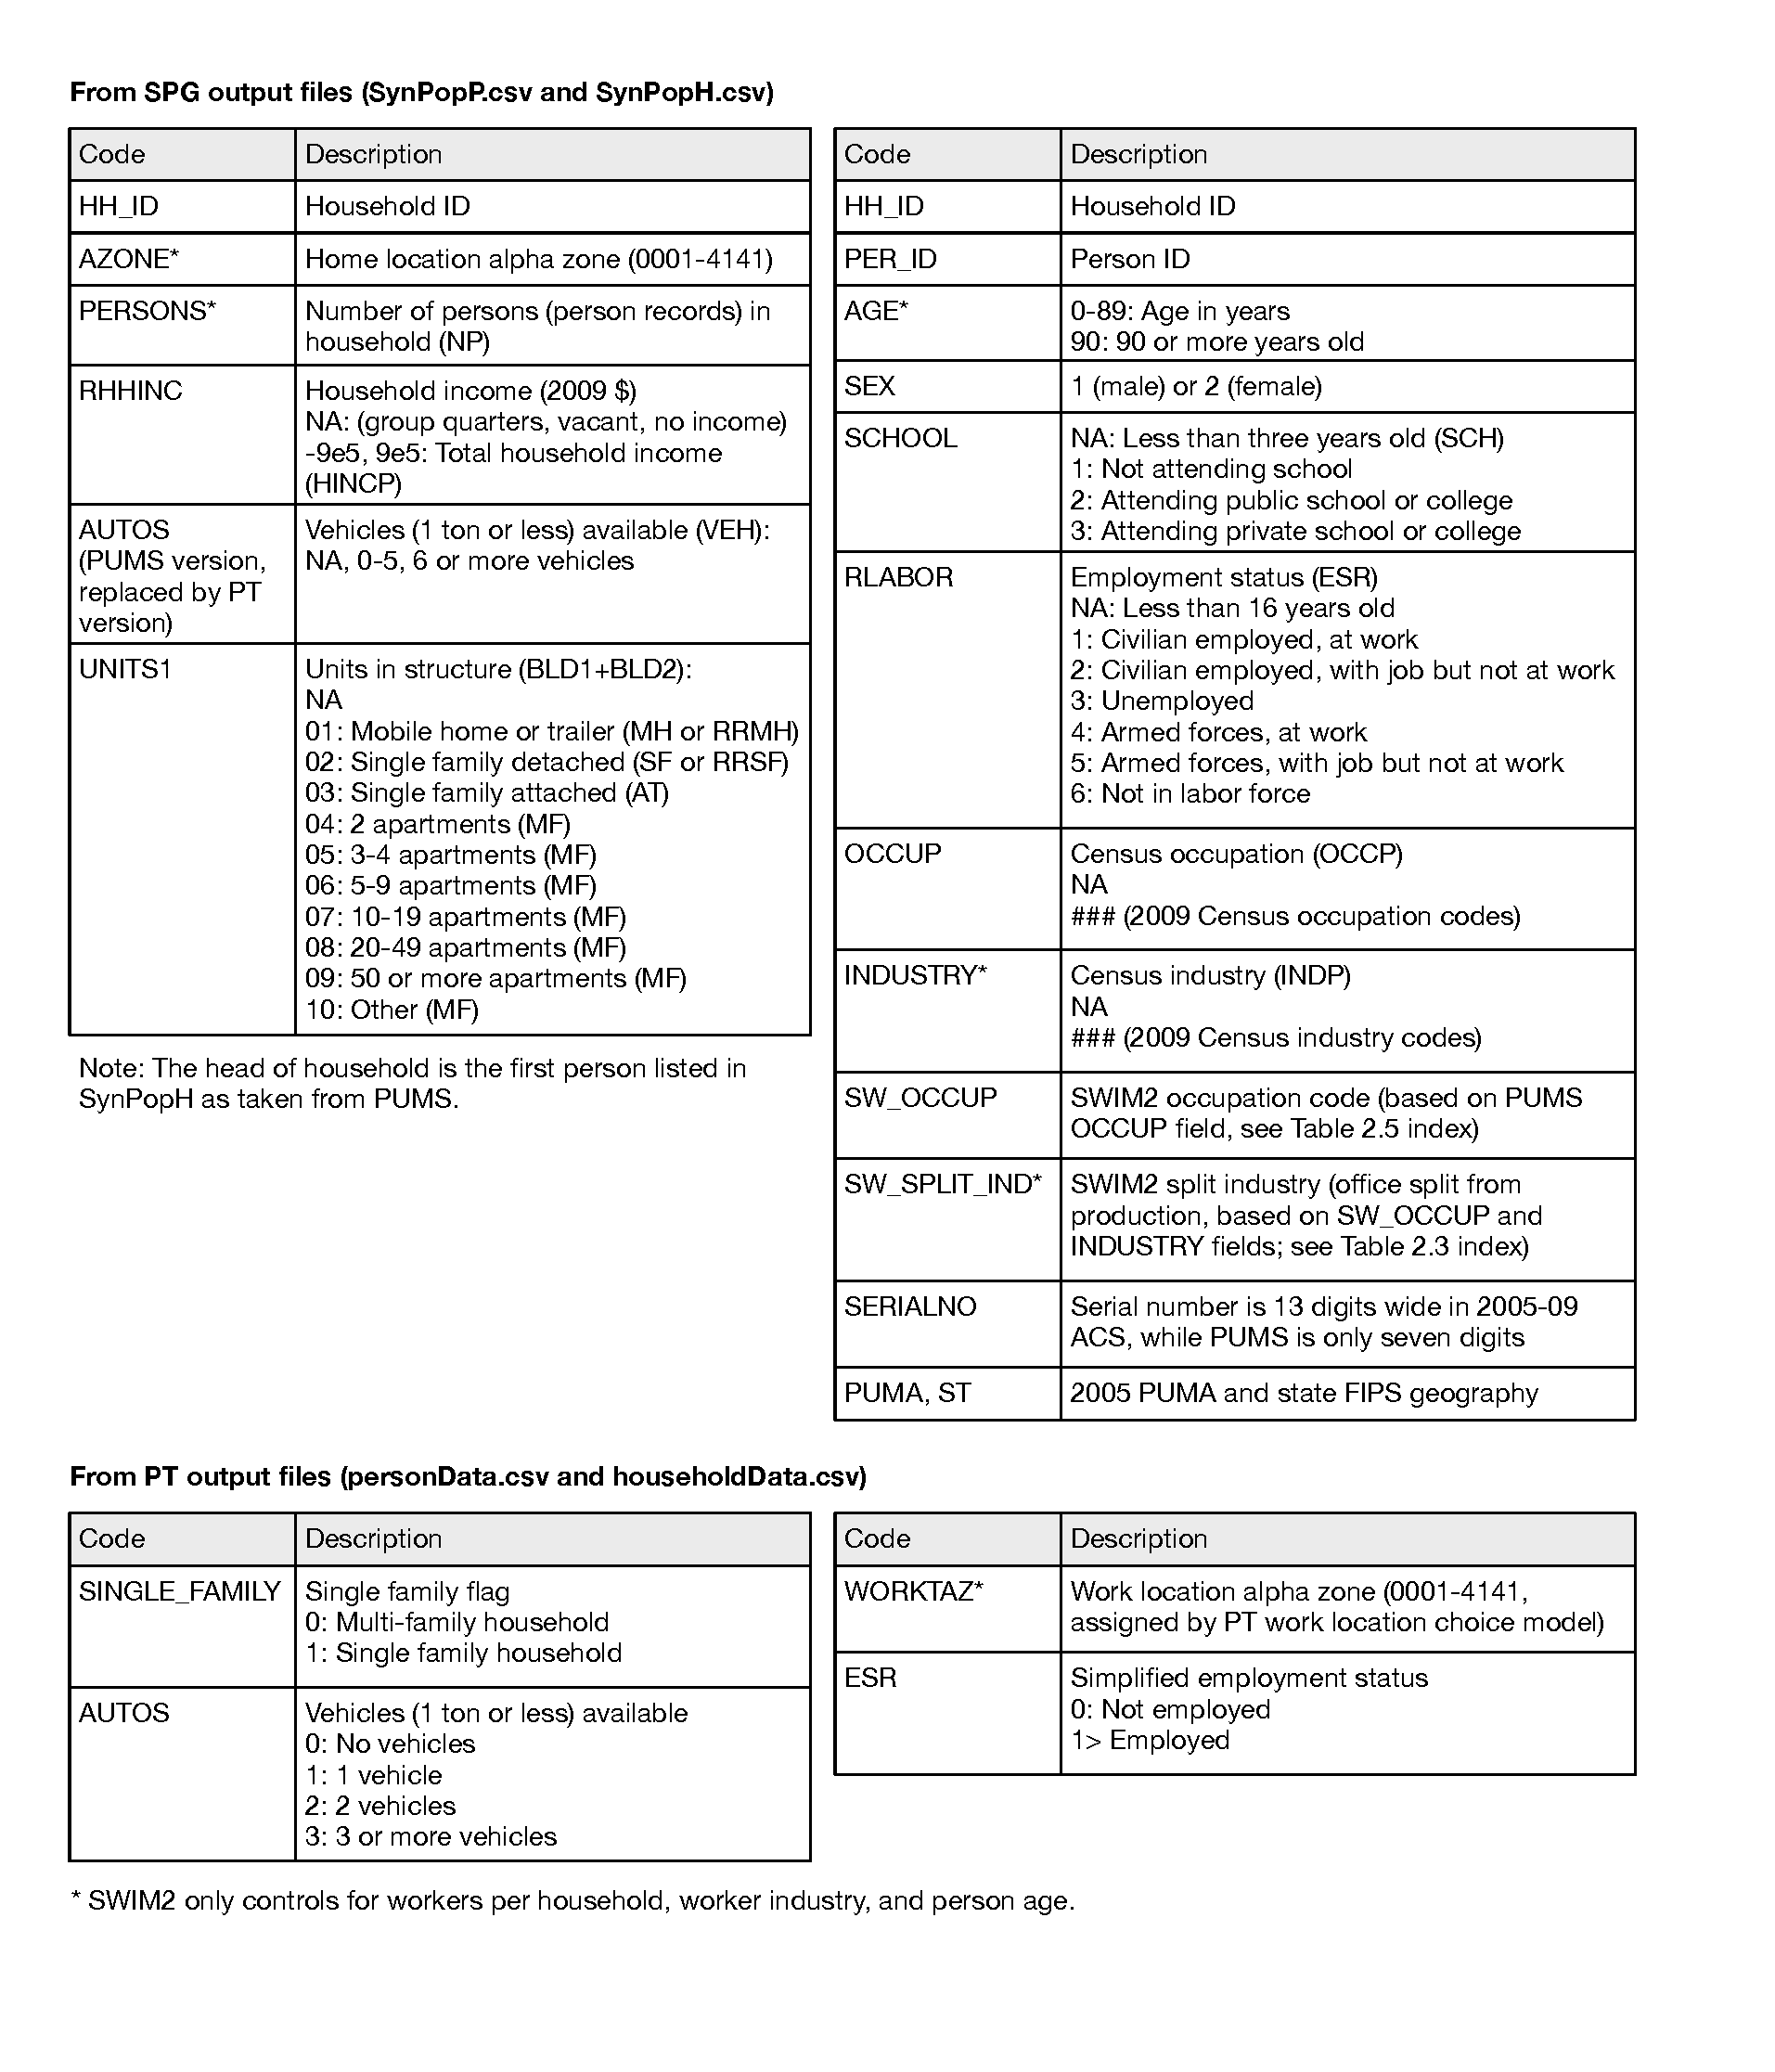
\includegraphics[width=7in]{overview/synthetic-attributes}
\caption{Synthetic population household and person attributes}\label{fig:synthetic-attributes}
\end{figure}

\noindent Other variables that could be retained in the 1990 Census PUMS household record include:
\begin{quote}
SERIALNO, GQINST, ROOMS, TENURE, ACRE10, ONEACRE, YRMOVED, COMMUSE, VALUE, RENT1, MEALS, BEDROOMS, WATER, SEWAGE, YRBUILT, CONDO, AGSALES, RTAXAMT, RFARM, RFAMINC, RWRKR89, RHHFAMTP, RNATADPT, RSTPCHLD, RFAMPERS, RNRLCHLD, RNONREL, R18UNDR, R60OVER, R65OVER, RSUBFAM
\end{quote}

\noindent Other variables that could be retained in the 1990 Census PUMS person record include:
\begin{quote}
SERIALNO, RELAT1, RACE, MARITAL, RSPOUSE, RAGECHLD, YEARSCH, MOBILITY, MILITARY, DISABL1, DISABL2, MOBILLIM, HOURS, WORKLWK, MEANS, RIDERS, DEPART, TRAVTIME, TMPABSNT, LOOKING, AVAIL, YEARWRK, CLASS, WORK89, WEEK89, HOURS89, REARNING, RPINCOME, INCOME1
\end{quote}
 
\section{Running the SWIM2 system}
The SWIM2 system runs on two dedicated computer servers housed at the Transportation Planning Analysis Unit at ODOT. The modeling system is run using a Python script that sets up the directory structure required, calls each of the component modules, and runs the model through time.\footnote{The function was formerly carried out using a model runner system graphical user interface (MrsGUI), which facilitated password-protected remote desktop access to a computing cluster at the State Data Center. MrsGUI executed a series of remote commands required to run the model, to include building scenarios, running the model, providing real-time status information, running post-processing metrics, and transfer of outputs and log files to a local computer.} The SWIM2 User's Guide contains more information on the computing cluster, program installation, file preparation, and instructions for running the model and post-processing scripts. The rest of this section provides an overview of the model directory structure and key functionality of the model runtime process.

All of the SWIM2 components except for the CT module are written in the Java programming language, and makes use of parallel processing where possible to reduce model runtimes. The CT module is written in the R statistical language\footnote{\url{https://www.r-project.org}}, as are some of the post-processing scripts used elsewhere in the model. Finally, the PTV Group's VISUM platform\footnote{\url{http://vision-traffic.ptvgroup.com/en-us/products/ptv-visum/}} is used for highway and transit assignments. It replaces the transport supply (TS) module developed for earlier version of SWIM2. TS was designed to facilitate micro-assignment of trips, whereby the traveler and trip characteristics could be retained through a standard macroscopic traffic assignment. This functionality was no longer needed when it was decided to adopt the aggregate PECAS framework, discussed in Chapter \ref{sec:aa-module-chapter}, in place of evolutionary microsimulated households and firms. Replacing the TS module with VISUM enables faster model runtimes, and reduces the number of modules that the SWIM team must support and maintain.

\subsection{Directory structure}
The directory structure for the SWIM2 system is shown in Figure \ref{fig:directory-structure}. The structure separates user-modified inputs, parameters, base year inputs, from scenario outputs, simplifying the user interface, and facilitating scenario backup and archiving. 

\begin{figure}
\centering
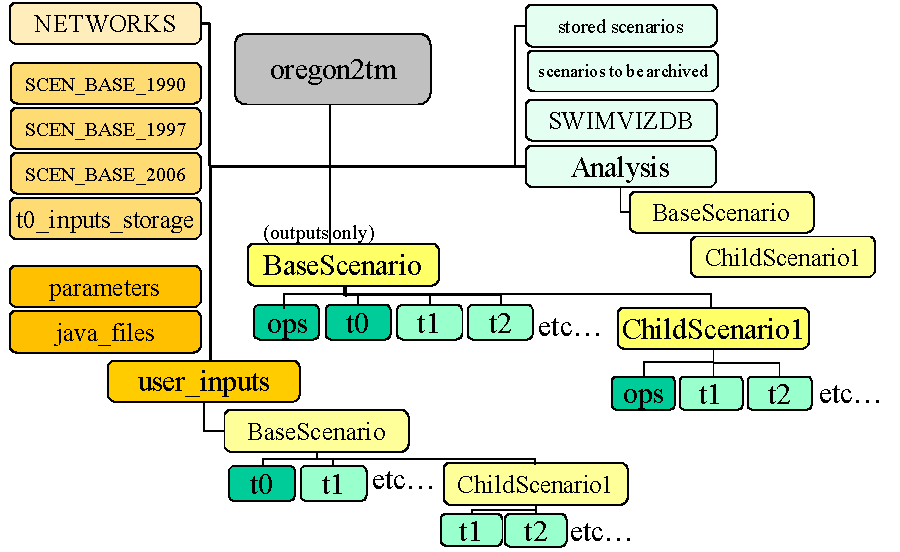
\includegraphics[width=5in]{overview/directory-structure}
\caption{SWIM2 directory structure}
\label{fig:directory-structure}
\end{figure}

After a scenario is created, all input files and code necessary to run the model are split among three folders: parameters (fixed after calibration), java\_files (fixed software and configuration files) and user\_inputs (select set of user-modifiable files). The user\_inputs directory has sub-folders for each scenario and within each folder, a sub-folder for each year. The Analysis folder also has this scenario-year sub-folder structure. A user can set up ``child'' scenarios that hinge off of base or ``parent'' scenarios. Child scenarios, like base scenarios, contain their own year sub-folders that house all child model user\_inputs and outputs (including potential bootstrapped outputs copied in when the child scenario was created). Output scenario-specific log files and the command file used in each run are housed in the scenario's ops folder. This folder structure is described in more detail below.

Each run of the model has its own base scenario directory structure which is a complete reference scenario run and stores full model outputs. Inputs would reside in the user\_inputs, parameters or as the output of other modules, in the current or previous year directory for the scenario. The Base Scenario/t0/ folder files would duplicate the t0\_inputs\_storage folder files, copied into the Base Scenario when created. Child scenarios would simply require the user to create a Child Scenario folder in the user\_inputs folder with appropriate file changes from the base year stored in its scenario-year sub-folders. Running the model would generate the model outputs in the sub-folders of the Base Scenario or Child Scenario.

Some files are constant over time and therefore the modules will always look in the base year t0 directory (or common reference directory) unless directed differently in the properties file. For example, a file of vehicle occupancies used by VISUM that applies to all years would be saved in the t0 VISUM subdirectory. If for vehicle occupancies changed in future year t$n$, for example, a separate file with the new occupancies is placed in the user\_inputs scenario t$n$ subdirectory along with a globalTemplate.properties file (indicating t$n$ path to this file references). This latest occupancy file would then remain in effect until the end of the simulation or until a later year properties file was found. 

\subsection{SWIMVIZ database and visualization tool}
SWIMVIZ was developed to dynamically visualize and inspect core multi-year SWIM2 model results and better understand SWIM2 operations. It contains both a database (SWIMVIZ DB) and an Adobe Flash application tool (SWIMVIZ tool). 

The SWIMVIZ DB conveniently organizes the core output data for all years of a scenario. Data are organized in a few tables at the beta zone level. This standardized format facilitates further output processing using the SWIMVIZ tool or other scripting, such as using SQLite and R statistical software. The key tables are listed in Table \ref{tab:swimviz-key-tables}, with more detail available in the SWIMVIZ DB documentation.

\begin{table}[!t]
\centering
\caption{Key SWIMVIZ database tables created during each model run}\label{tab:swimviz-key-tables}
\begin{tabular}{l L{4.5in}}
\hline
Table & Description \\
\hline
ACTIVITYLOCATIONS & The quantity of activity generated by beta zone, such as industry activity (2009 dollars), households, and employment. \\
\gray BUYSELLMATRIX & The commodity flows from the AA module between beta zones, including the dollar flow of labor, goods and services. \\
EXCHANGERESULTS & Information on the exchange of commodities (goods, services, labor and floorspace), such as the quantity of demand and supply, price, etc. \\
\gray FLR\_INVENTORY & ALD beta zone floorspace inventory and zoning capacity by type. \\
DC\_LOGSUM & Average logsums by beta zone, trip purpose, and market segment. \\
\gray TRIPS\_SDT & Short-distance person trips and trip distances by origin beta zone for each time period. \\
TRIPS\_SDT\_Home & Same as TRIPS\_SDT, except trips are aggregated by person trip household home beta zone origin rather than trip origin. \\
\gray Trips\_LDT & Long-distance person trips and trip distances by origin beta zone for each time period. \\
TRIPS\_LDT\_Home & Same as TRIPS\_LDT, except trips are aggregated by person trip household home beta zone origin rather than trip origin. \\
\gray Trips\_CT & Commercial truck trips and trip distances by origin beta zone and commodity for each time period. \\
TRIPS\_CT\_Home & Same as Trips\_CT, except trips are aggregated by beta zone of truck tour origin, rather than trip origin. \\
\gray TRIPMATRIX & Combined trip matrices for each beta zone origin-destination pair, time period, and mode from SDT, LDT, and CT aggregated to common modes/truck classes. \\
LINK\_DATA & Network assignment results (volumes, etc.) for each time period. \\
\gray SKIM & Travel distance, time, tolls for each beta zone origin-destination pair for peak and off-peak, auto and truck. \\ 
MODELWIDE & Various modelwide data, typically associated with the NED module. \\
\hline
\end{tabular}
\end{table}

A SWIMVIZ Micro database stores the synthetic population (persons and households from SPG), as well as detailed tour and trip information for person (from PT) and trucks (from CT). The key tables included in this database are shown in Table \ref{tab:swimvia-micro-tables}, with more detail available in the SWIMVIZ DB micro documentation and SWIM2 User's Guide.

\begin{table}
\centering
\caption{Key SWIMVIZ microdata tables created during each model run}\label{tab:swimvia-micro-tables}
\begin{tabular}{l L{4.8in}}
\hline
Table & Description \\
\hline
HH & Households in the model and their key attributes, including description of any long distance tours. \\
\gray PER & Persons in the model and their key attributes, including industry, work status. \\
TOUR\_LDT\_MICRO & All long distance tours in the model, including their purpose, mode origin and destination zones, times and party size. \\
\gray TRIP\_LDT\_MICRO & All long distance vehicle trips in the model, including their purpose, mode origin and destination zones and times. \\
TOUR\_SDT\_MICRO & All short distance tours in the model, including their purpose, mode origin and destination zones and times. \\
\gray TRIP\_SDT\_MICRO & All short distance person trips in the model, including their purpose, mode origin and destination zones and times. \\
TRIP\_CT\_MICRO & All short and long distance truck trips in the model, including commodity, carrier type, weight origin and destination zones and times. \\
\hline
\end{tabular}
\end{table}

During model setup the user can flag that a scenario produce one or both of these VIZ DBs. Then a SQLite database for each year of the scenario is created after the model run completes and compiled into a master scenario sqlite database that contains all years. A zipped version of the multi-year SWIMVIZ DB is copied to the ODOT FTP site facilitating remote users in obtaining this data.

\subsection{Application Orchestrator (AO) component}
The AO module is a collection of components that directs the flow of the full SWIM2 Model. The key components of AO include:
\begin{itemize}
\item The Distributed Application Framework (DAF)
\item Launching components (using Ant and ApplicationOrchestrator.java and FileMonitor.java)
\item Monitoring progress (using Logger.java)
\end{itemize}

\noindent The SWIM2 components are either monolithic and distributed. A monolithic application is one that is run on a single machine, more specifically inside a single Java Virtual Machine (JVM), also referred to as a node. The NED, ALD, AA, SPG1, and SPG2 components are monolithic. A distributed application is one that is run on multiple machines or inside several JVMs, or in other words on more than one node. A collection of nodes that communicate with one another is called a cluster. PT and CT are examples of distributed applications. These applications could be run monolithically, but distributing the process over multiple nodes significantly decreases their run times. The code is broken up into tasks that can be performed simultaneously on different nodes for a different set of objects. For example, a task might calculate the composite buying and selling utilities for each commodity. If distributes across eight nodes, for example, the composite utilities can be calculated in parallel. There is some coordination required when separating code into tasks, as the data has to once again be combined. The Distributed Applications Framework Version 2 (DAF2) provides this coordination. The CT component uses the doParallel package in the R statistical language to achieve the same effect.

The DAF code was written to handle the distribution of an application over multiple nodes. It provides the communication mechanism, a messaging system, that allows the nodes to send messages to tasks on other nodes, receive messages and to listen for messages from other nodes. Tasks listen for messages to arrive in a work queue associated with that task. As soon as work arrives it is processed, and a return message is usually sent. DAF also provides methods to start and stop all nodes in a cluster from a single node and to start an application from a node outside of the cluster. 

A daf.properties file is used to define a DAF cluster. A cluster can be a single machine that runs multiple JVMs with one task per JVM, or perhaps five machines running five JVMs with ten tasks running in each JVM. Machine memory is the biggest constraint, as each JVM uses up to 8 gigabytes (GB) or more of memory. The daf.properties file describes only the nodes, and therefore the cluster is defined independent of the application that will be run on it. An application may utilize all nodes in a cluster or only a subset of them. An application-specific daf.properties file is therefore also necessary to describe each task that the application will perform and assign it to a particular node. The work queues are defined in the properties file where they are associated with a particular task and a particular node. MrsGUI codifies various set DAF configurations.

The structure of a DAF application is illustrated in Figure \ref{fig:daf-example}. It shows how a component might be distributed over three nodes. For the example described above the tasks might include a master task, a CUWork task (calculating the composite utilities of buying and selling a particular commodity in a particular exchange zone), a SDWork task (calculating the surplus and its derivative of a particular commodity in a particular exchange zone), two result processing tasks, and associated work queues.

\begin{figure}
\centering
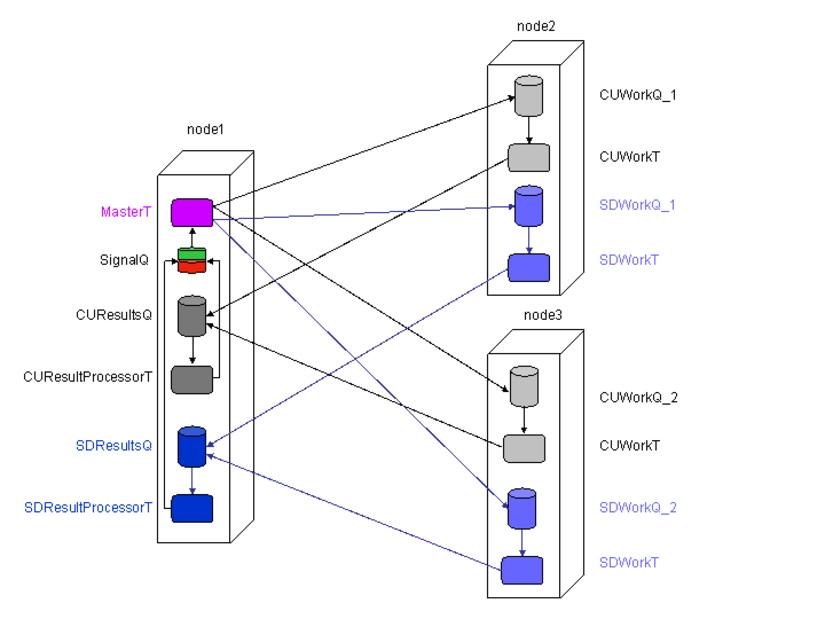
\includegraphics[width=5in]{overview/distributing-pi-module}
\caption{Distributing component flows}
\label{fig:daf-example}
\end{figure}

\subsection{Launching a component}
The launch of each component is currently being done using Python ANT Substitute (PANTS), a program which was created to replace the previous component launching program, Ant. One of the benefits of PANTS are that it allows tasks to be specified in Python (as opposed to XML, which is used by Ant), which allows a natural program flow to be specified using standard programming idioms. Another advantage is that it stores an entire run sequence in a database, which allows the model run's sequence position to be determined, as well as allowing a run to be continued if it was stopped. PANTS uses a definition file written in Python, which specifies targets which are accessible to the user. These targets build up a model sequence, which is then loaded into a database and finally the sequence is executed using database queries to determine each step

In the case of the monolithic components the PANTS target (e.g., runED, runALD) located in the TlumipDef.py file starts a new JVM on a machine in the cluster, instantiates the AO object inside it, and passes to it the name of the component (e.g., NED) to be started. AO then simply creates an instance of the named component and calls its runModel method. This assumes that the constructor of that component will read the appropriate properties file and configuration files. Properties files contain runtime information, such as the name of input files. Configuration files hold the things that do not change, such as internal parameter values. The component will then handle the rest of the processing. Each module component will clean up after their run and communicate with other components via data files and thus, does not return data structures or other information to the orchestrator. 

A distributed component is also launched using a PANTS target so that the AO is created inside its own node, as discussed above. For the distributed components, however, this node must start other nodes both on its local machine as well as nodes on remote machines in the cluster. A FileMonitor object is the mechanism by which the Orchestrator object communicates with DAF. The FileMonitor class uses a simple text file as a command file, and serves as a central command station. Each machine in a DAF cluster will create a FileMonitor object in a small JVM. This object monitors the command file for changes. When a change in the lastDateModified attribute is detected, the FileMonitor reads the contents of the file and executes the command found therein. 

Thus, to start a distributed application, the AO object first writes StartNode into the command file. AO waits for a short time and then writes ``StartCluster'' into the command file, overwriting the previous command. The orchestrator again waits and then writes the name of the application that is supposed to run into the command file. The FileMonitors, detecting the changes, execute the appropriate code on their machine. AO then waits for the appearance of a ``done'' file that will be written by the application when it has finished executing. When the done file appears, AO will write ``StopNode'' into the command file and the FileMonitors will stop the Java processes running on the machines.

%For more information on the FileMonitor class, see additional reference on this topic [3]. 

\subsection{Logging}

AO uses logging statements generated by the individual modules to provide feedback to the users as to the module's progress. These log statements can be directed to the console or to a file as specified in a logging.properties that is shared by all components. The following logging output is generated automatically and written to the Scenario /ops directory during a model run:
\begin{itemize}
\item Main\_event.log (the main process log file)
\item Node[node number]\_event.log (the log file for the DAF node on computer [node number])
\item Bootstrap\_server\_node[node number].log, bootstrap\_client.log, fileMonitor\_event.log (logs related to the inner workings of the DAF components)
\item Global\_status.log (a global status log file)
\item Status.log (a module-level status log file)
\end{itemize}

\noindent In addition to the log files, at the end of each run, a Java program is run which reads the log files and summarizes the run at both a global and module level. The files created by the process (also placed in the /ops directory) include ModuleSummary.csv (an overall summary of the runtimes of the various modules) and PtIterationSummary.txt (a summary of the PT module). 
 
\section{Calibration approach}\label{sec:calibration-approach}
A three-stage process is used to develop the values for the parameters in the various modules in the model:
\begin{itemize}
\item In Stage 1 (\textbf{S1}) values are developed for certain parameters in each module separately. The intention is that these first-stage values for the S1 parameters will remain fixed as the model development and calibration work progresses. When suitable observations of system behavior are available, statistical methods are used to estimate appropriate values for S1 parameters. In some cases, only a single observation is available and direct methods are used to provide values. At this point it is not necessary that the modules can be run: the components of the modules are being ``assembled'' and the outputs of the modules are not yet being considered.
\item In Stage 2 (\textbf{S2}) initial values are established for all of the parameters that are not S1 parameters, considering the fit of each module in isolation. The fit for a given module concerns specified targets for outputs from the module, so the module needs to be run in order for it to provide these outputs. Thus, a full set of required inputs for each module needs to be developed, including all those provided by other modules and all those provided exogenously. In order to obtain reasonable values for the S2 parameters, these inputs need to be consistent with the specified targets, representing conditions similar to those that gave rise to the targets.
\item In Stage 3 (\textbf{S3}) the initial values established for certain sets of the S2 parameters are revisited for all of the modules simultaneously, considering the fit of all modules together. These are evaluated with the full model running, so that inputs to the modules are coming from the other modules in the way they would for a model run. The second and third stages together constitute a Bayesian updating process for these S3 parameters. Ideally, all parameter values would be revisited, but this is not possible for practical reasons. A weight sensitivity matrix can be used to explore the remaining lack-of-fit for the entire model, which can help identify the parameters to focus on in the third stage and which may lead to small changes in the details of the model design and specification.
\end{itemize}

The development of the values for the S1 and S2 parameters, in the first and second stage of the parameter development process, is described for each module in the subsequent chapters. This includes a description of the work done to get each module running, as required, using input values and certain interim values for parameters as required. 

Certain initial values for the S2 parameters are revisited in Stage 3 of the parameter development process. Stage 3 includes the work necessary to get the entire set of all SWIM2 components running in order to provide a fully integrated modeling system. All SWIM2 components, excluding the optional selected link (SL) component, have completed this three-step calibration process.
